\begin{frame}\frametitle{Corrections to the Calibration of MODIS Aqua Ocean Color Bands Derived From SeaWiFS Data} 
\begin{description}
    \item[Authors] Gerhard Meister, Bryan A. Franz, Ewa J. Kwiatkowska, Charles R. McClain
    \item[Summary] \scriptsize A new calibration method was needed to correct a problem affecting the Moderate Resolution Imaging Spectroradiometer, MODIS Aqua’s, ability to provide accurate ocean color data. The system uses bands 8-14 to detect water leaving radiances from the Earth’s surface. The problem affected temporal information collected for wavelengths between 412-443 nm. Prior to the calibration issues, the MODIS Calibration and Support Team (MCST) used onboard calibrators and lunar irradiances to sufficiently calibrate the MODIS systems. Now, the calibration methods are based on the Ocean Biology Processing Group’s (OBPG) calibration solution for MODIS Terra, which experienced a similar problem. In this method, the MODIS system is cross-calibrated with SeaWiFS to recharacterize the data to correct for the temporal trend error. Now, ocean color data is made with SeaWiFS and MODIS Aqua data merged together. Each data set is processed on its own and then reconfigured.
\end{description}

  \note[item]{Include notes and talking points here.}
  \note[item]{There can be more than one note.}
\end{frame}

\begin{frame}\frametitle{Corrections to the Calibration of MODIS Aqua Ocean Color Bands Derived From SeaWiFS Data} 


\begin{columns}
\begin{column}{0.5\textwidth}
    \begin{center}
    \textbf{\scriptsize SEAWIFS SWATHS}
    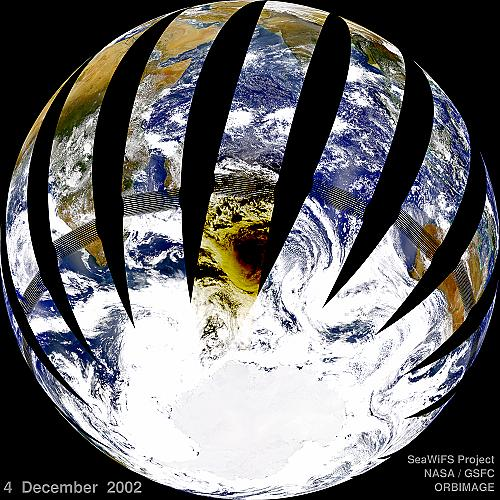
\includegraphics[width=\textwidth,height=0.8\textheight,keepaspectratio]{N7Pw7r}

    \tiny \textbf{Source:} \url{http://epod.typepad.com/.a/6a0105371bb32c970b0115714d7c00970c-500wi}
    \end{center}
\end{column}
\begin{column}{0.5\textwidth}  %%<--- here
    \begin{center}
    \textbf{\scriptsize MODIS AQUA PREDICTED PATHS}
    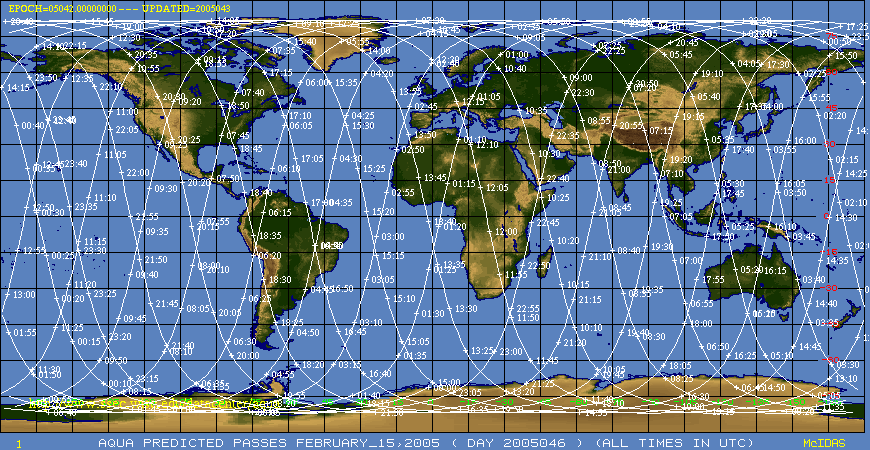
\includegraphics[width=\textwidth,height=0.8\textheight,keepaspectratio]{kVvOUr}

    \tiny \textbf{Source:} \url{https://nsidc.org/sites/nsidc.org/files/aqua_tracks.20050215.gif}
    \end{center}
\end{column}
\end{columns}

\end{frame}
